\chapter{Review odborného članku}

Název článku: Aircraft Control System Using LQG and LQR Controller with Optimal
Estimation-Kalman Filter Design \\
Autoři článku: Labane Chrif, Zemalache Meguenni Kadda \\
Odkaz na článek:
\href{https://www.sciencedirect.com/science/article/pii/S1877705814011771}{www.sciencedirect.com} \\
\textbf{Seznam Příloh:} aircraft.pdf 

\section{Review}

Tato práce se zabývá implementaci řízení letadla pomocí metod \textbf{LQG}
(Linear–Quadratic–Gaussian control) a \textbf{LQR} (Linear–Quadratic regulator) pomocí
nástrojů Matlab/Simulink. Kombinace metody řízení LQR a \textbf{Kálmánová
filtra} umožnuje
lepší odhad parametrů, získaných ze sensorů a následovné řízení letadla.



V oblastech letectvy nároky na systémy řízení jsou násobně větší vzhledem
k účinnosti a spolehlivostí systémů. S rostoucí požadavky na řízení a
autonomnost letadel jedním řešením je zvětšení čísla senzoru a akčních členu.
Což má za následek zvětšení ceny výrobku. Nicméně moderny přístupy k řízení
systému máji byt schopny pracovat s mnoha vstupní a výstupní parametry. Jedním
z řešení je LQG, který je vhodný pro použiti v praktických úlohách, kde systém
ovlivněn rušením a šumem měřeni.


Pro řízeni letadla jsou 3 dostupné rotace, které umožnují změnit směr letu
letadla. To jsou \textbf{Pitch}, \textbf{Roll} a \textbf{Yaw}. Řízení dále se dělí na podélný směr a boční
směr.


Dynamika v podélným směru (longituadinal dynamic) ve stavové representace vypadá
nesledující:

\begin{equation}
    \begin{bmatrix}
        \dot{w} \\
        \dot{q} \\
        \dot{\theta} 
    \end{bmatrix} 
    = \textbf{A}   
    \begin{bmatrix}
        w \\
        q \\
        \theta 
    \end{bmatrix} 
    + \textbf{B} [\delta_e] \\
\end{equation}

\begin{equation}
    y = \textbf{C}
    \begin{bmatrix}
        w \\
        q \\
        \theta 
    \end{bmatrix} + \textbf{D}
\end{equation}

Matice \textbf{A}, \textbf{B}, \textbf{C}, \textbf{D} lze dohledat v članku.


Dynamika v bočním směru (lateral dynamic) ve stavové representace má tvar:


\begin{equation}
    \begin{bmatrix}
        \dot{\beta} \\
        \dot{p} \\
        \dot{r} \\
        \dot{\phi} 
    \end{bmatrix} 
    = \textbf{A}   
    \begin{bmatrix}
        \beta \\
        p \\
        r \\
        \phi 
    \end{bmatrix} 
    + \textbf{B}
    \begin{bmatrix}
        \delta_a \\
        \delta_r
    \end{bmatrix} 
\end{equation}

\begin{equation}
    y = \textbf{C} 
    \begin{bmatrix}
        \beta \\
        p \\
        r \\
        \phi 
    \end{bmatrix} + \textbf{D}
\end{equation}

Matice \textbf{A}, \textbf{B}, \textbf{C}, \textbf{D} lze dohledat v članku.

LQG regulátor se skládá z filtru Kalmana a LQR regulátora zařazeních za sebou,
jak znázorňuje následující diagram \ref{fig:lqg_control}. 
\begin{figure}[ht]
    \centering
    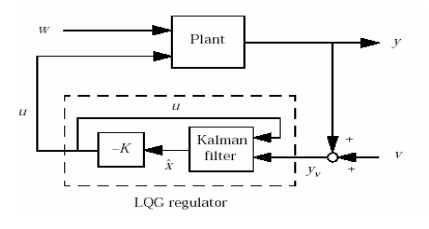
\includegraphics[width=0.6\textwidth]{lqg_control.png}
    \caption{Plant model in Simulink.}
    \label{fig:lqg_control}
\end{figure} \\

Pro přenos regulátora platí:

\begin{equation}
    \frac{d}{dt}\hat{x} = [A - LC - (B - LD)K]\hat{x} + Ly_v \\
\end{equation}
\begin{equation}
    u = - Kx
\end{equation}


Soustava obsahující rušeni je doplněna o $w$ a $v$, které představuji bily sum:
\begin{align}
    \dot{x} = Ax + Bu + Gw \\
    y_v = Cx + Du + Hw + v
\end{align}


Při návrhu LQR regulátoru uživatel na základě zkušeností odhaduje matice $Q$,
$N$, a $R$ které představuje rychlost, se kterou požadovaný parametr se přibližuje
k žádané poloze a také úsilí, které regulátor musí vykonat pro dosazeni této
polohy. LQR regulátor pracuje se znalostí celého stavového vektoru. Ale ve
většině případu nejsme schopny měřit cely stavový vektor $x$. Proto je nutné
použití Kálmánův filtr, který, pokud systém pozorovatelný a řiditelný, je
schopný tento stavový vektor odhadnout.


Při návrhu Kálmánova filtru počítáme že systém obsahuje určitou míru rušení (v
případě letadla to může způsobit vítr, nebo změny v hustotě vzduchu, které
vyvolá vibrace) a také měření ze sensorů obsahuje šum. Hlavním cílem je navrhnou
Kálmánův filtr tak aby odhad parametrů byl co nejpřesnější.


Výsledky simulace znázorněny v článku.

\section{Krirické zhodnocení}

Z uvedených výsledku lze konstatovat že řízení LQG je schopné řídit pitch angle,
roll angle a sideslip angle letadla. Přítomnost Kálmánova filtru zaručuje
optimální odhad a rekonstrukce parametru stavového vektoru pří výskytů bílého
sumu.

Článek vyžaduje určitou míru znalosti v problematice dynamiky letadla. Většina
koeficientu v kapitolách 2. a 3. vyžaduje studium dalších zdrojů. Při čtení mě
přispěla presentace \\
\href{http://adl.stanford.edu/sandbox/groups/aa241x/wiki/e054d/attachments/c53d7/Aircraft%20Flight%20Dynamics%202015_04_13.pdf?sessionID=62f441d3fcc6b4014c66ce9aa5d732f561008d30}{adl.stanford.edu/}
tykající základní informace o dynamice letadla.
Nicméně následující kapitoly dostatečně přehledné a informativní. Implementace
diskrétního Kalmana vyžaduje od čtenáře znalost použiti přechodů v Simulinku
mezi systémem se spojitým časem a diskrétním. Toto lze zrealizovat například blokem Zero-Order-Hold.
